%\section{Introduction}
%\label{s:intro}

{\bf Executive summary.} \emph{CryptDB} is a DBMS that provides
provable and practical privacy in the face of a compromised database
server or curious database administrators. CryptDB works by executing
SQL queries over encrypted data.  At its core are three novel ideas:
an \textit{SQL-aware encryption strategy} that maps SQL operations to
encryption schemes, {\em adjustable query-based encryption} which
allows CryptDB to adjust the encryption level of each data item based
on user queries, and \textit{onion encryption} to efficiently change
data encryption levels.  CryptDB empowers the server to execute only
queries that the users requested, and achieves maximum privacy given
the mix of queries issued by the users. The server fully evaluates
queries on encrypted data and sends the results back to the client for
final decryption; clients don't perform any query processing and
client-side applications run unchanged. Our evaluation shows that
CryptDB has modest overhead: on the TPC-C benchmark on Postgres,
CryptDB reduces throughput by $\tput$ compared to regular
Postgres. Moreover, CryptDB does not change the innards of existing
DBMSs: we realized the implementation of CryptDB using client-side
query rewriting/encrypting, user-defined functions, and server-side
tables for public key information.
%As such, CryptDB is portable;
%porting CryptDB to MySQL required changing $86$ lines of code, mostly
%at the connectivity layer.

{\bf Motivation and problem.}  Theft of sensitive private data is a
significant problem~\cite{prc:breaches}.  DBMSs are an especially
appealing target for attackers, because they often contain large
amounts of private information.  When individual users or enterprises
store their sensitive data in a DBMS today, they must trust that the
server hardware and software are uncompromisable, that the data center
itself is physically protected, and assume that the system and
database administrators (DBAs) are trustworthy.  Otherwise, an
adversary who gains access to any of these avenues of attack can
compromise the entire database, as has been documented in a number of
published reports of data thefts~\cite{prc:breaches}.
%(and presumably
%there are more compromises that have not been publicized).

These stringent security requirements are also at odds with
cost-saving measures such as the consolidation of DBMSs belonging to
different business units into a common enterprise-wide IT
infrastructure, moving databases into a public cloud, or outsourcing
DBA tasks.  In fact, ``lack of trust'' is an oft-quoted primary
concern about moving DBMSs to more cost-effective cloud
infrastructures.  Moreover, thanks to high-profile thefts of social
security identifiers, credit card numbers, and other personal
information from various online databases, these concerns are
increasingly being reflected in the law as well: for instance, recent
legislation requires that all databases containing personal data about
Massachusetts residents be encrypted~\cite{Masslaw}.

% A significant barrier to deploying database systems in the cloud is
% the perceived lack of privacy, which in turn reduces the degree of
% trust users are willing to place in such deployments. If clients were to
% encrypt all the data stored in the cloud database, and if the data
% were decrypted only on client-controlled machines, then privacy
% concerns would largely be eliminated. Similarly, even in so-called
% private clouds inside enterprises, users often desire the ability to
% store data and run queries in data centers without trusting the
% database and system administrators with the content.

{\bf Our approach: SQL query processing over encrypted
  data.}  We introduce {\em CryptDB}, a practical relational DBMS that
provides provable privacy guarantees without having to trust the DBMS
server or the DBAs.  In CryptDB, unmodified DBMS servers store {\em
  all} data in encrypted formats, and execute SQL queries over
encrypted data without having access to the decryption keys.  CryptDB
works by intercepting and rewriting all SQL queries in a frontend to
make them execute on encrypted data, by encrypting and decrypting all
data, as well as changing some query operators, while preserving the
semantics of the query.  The frontend has access to the encryption
keys for the entire database.  By not giving the DBMS server access to
the decryption keys, CryptDB greatly reduces trust requirements for a
DBMS server.  For example, CryptDB can alleviate privacy concerns when
outsourcing databases to a cloud computing
environment~\cite{xeround-blog}, such as Amazon's AWS, Microsoft's SQL
Azure, or Google's AppEngine, or when outsourcing the work of DBAs.
CryptDB can also prevent privacy breaches due to curious
administrators
%~\cite{chen:gmail-snooping} 
or compromised DBMS servers.

% \hb{Less related work here.}
% While early proposals attempted to enable SQL processing over encrypted
% data~\cite{sqlOverEncryption}, their privacy mechanisms were mostly heuristic,
% required a significant rewrite of the DBMS design, relied on considerable
% client-side processing, and did not support certain SQL queries. More recent
% literature~\cite{Dawn-Song-Search-2000, Chang04privacypreserving,
% queriesEncryptionBoneh,
% amanatidis-boldyreva-o'neill, Yang-privacy-preserving-queries,
% encrypt-for-secure-outsource, private-query-multi-user-for-searchable} has
% developed cryptographic tools for searching keywords on encrypted data and has
% proposed using these tools to process SQL queries on encrypted data. Although such
% work is a good first cut at the problem, it does not provide a
% comprehensive systems solution: they do not support many basic SQL queries (and
% mostly only support equality comparisons), some of them require significant
% client-side query processing, change the internal processing of a DBMS, and many
% of these schemes are too inefficient (requiring users either to build and maintain
% indexes or to perform sequential scans for every selection).


{\bf Challenges.}  There are three significant challenges in designing
and implementing a DBMS that operates on encrypted data.  The first
lies in supporting a wide range of SQL queries on encrypted data.
Unlike a simple encrypted data store, a DBMS must perform {\em
  computations} on encrypted data to execute SQL queries.  For
example, an SQL query may ask for the average salary of employees, for
the names of employees whose salary is greater than \$60,000, or for
the list of employees that share an office with more than two
colleagues.  Simply encrypting each row in the database with a single
key would not allow a DBMS server to execute such SQL queries without
access to the decryption key.

The second challenge lies in carefully defining ``privacy'' for an
untrusted DBMS, as well as coming up with a system design that
provably achieves that definition.  On the one hand, even if all of
the data stored on a DBMS server were encrypted, the server must be
able to perform certain operations on the rows, such as aggregations,
selections, and joins.  On the other hand, an adversary that
compromises a DBMS server may now learn information about the data,
such as relations between different rows in a table.  Thus, we need to
define privacy in a way that balances the need for server-side
computation with the need to minimize information revealed to the
server.

The third challenge lies in making an encrypted DBMS practical to use.
To provide good performance, an encrypted DBMS should impose tolerable
performance overheads on the server, but at the same time avoid
offloading SQL query execution onto the client.  To make an encrypted
DBMS easy to deploy, an ideal system would also require {\em no
  changes to existing DBMS server software}, so that it can take
advantage of more than four decades years of engineering and
optimization work, run on a range of commodity DBMS servers, and avoid
making any changes to applications.

{\bf Our solution.} We address these challenges in CryptDB's design
using three key ideas.  The first idea is an {\em SQL-aware encryption
  strategy}.  We observe that SQL queries are composed of primitive
operators, notably order comparisons, equality checks, and additions.
For most of these operators, we found existing encryption schemes in
which the operation can be performed on the ciphertext without knowing
the decryption key.  One exception is joins, for which no
cryptographic primitive existed; in this case, we developed a novel
cryptographic construction for privacy-preserving joins.  Given these
primitives, we encrypt each data item with encryption schemes that
enable the server to execute the necessary SQL operators on that data.
This approach is both efficient and practical, since the bulk of the
DBMS, including query planning, data layout, transaction coordination,
and the structure of the queries themselves, can remain the same, and
only individual SQL operators used by a query may need to change.

The second idea is {\em adjustable query-based encryption}, where
CryptDB dynamically adjusts the encryption level for each data item at
runtime, so as to achieve the maximum privacy level given the user's
queries.  In particular, CryptDB initially encrypts all data with the
strongest level of encryption, and, as the application issues SQL
queries, adjusts the level of encryption on the server, so that the
server can perform the classes of computations necessary for that SQL
query.  This model forms the basis of our privacy definition, ensuring
maximum privacy given the classes of computations required by the
queries presented to the DBMS.  It avoids the need to modify
application code to declare the necessary level of encryption ahead of
time.

\begin{figure}[t!] \centering 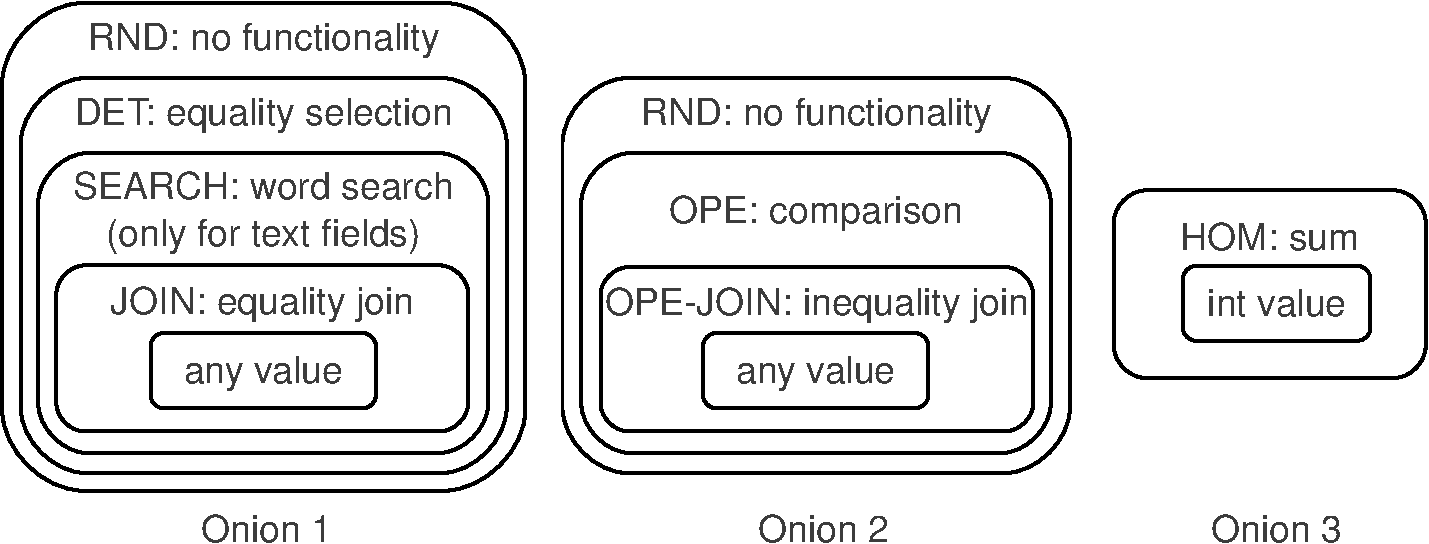
\includegraphics[width=3.3in]{storage.pdf}
  \caption{Onion layers of encryption and the classes of computation
    they allow.}
\label{fig:onion}
\end{figure}

The third idea is to implement adjustable query-based encryption by
encrypting each data item in an {\em onion of encryptions}, from
weaker forms of encryption that allow certain computations, to
stronger forms of encryption that reveal no information, as shown in
Figure~\ref{fig:onion} (the meaning of each layer to be presented in the talk). 
This approach allows CryptDB to efficiently adjust encryption levels on the server without having to re-encrypt
all data at the client.  For example, the outermost layer uses
randomized encryption, which guarantees that the server can learn
nothing about the data, aside from its length.  If the user issues an
SQL query containing {\tt WHERE id=5}, CryptDB sends the server an
{\em onion key} to decrypt the {\tt id} column to a deterministic
encryption level, where identical plaintexts have identical
ciphertexts. CryptDB then sends the server a deterministic encryption
of the constant $5$, allowing it to compute matching rows by only
revealing the necessary {\em relations between data items}, and {\em
  not revealing the actual data}, or other relations between data
items not used in this query.

% Privacy and practicality are 
% conflicting goals. At one extreme, theoretical approaches using fully homomorphic
% encryption~\cite{gentryVerifiable} support any general computation
%  on encrypted data and provide strong privacy guarantees (e.g., the DBMS
% does not even learn access patterns). Unfortunately,
% such approaches are prohibitively impractical; for example, performing a simple
% string search using homomorphic encryption is about a trillion times slower than without
% encryption~\cite{trillion}. At the other extreme, providing no privacy by
% keeping the data in the clear, provides high performance and functionality.

% The idea for achieving practical privacy is \textit{to
% allow the database server to process queries on encrypted data as it would do on clear
% data}; when the server needs to evaluate a predicate on two encrypted data
% items, we empower the server to do so.

% In this model, each query requires the server to perform a certain class of
% computations on stored data. For example,
% consider evaluating an equality filter such as \texttt{WHERE id = 5}. Given
% the encryption of $5$, say \texttt{x1c5a21}, the server needs to be able to
% figure out what rows in column \texttt{id} have an encryption of
% \texttt{x1c5a21}.  CryptDB allows the server to compute the set of rows whose
% {\tt id} column matches the given ciphertext, but does not reveal to the
% server the original values, or what plaintext \texttt{x1c5a21} corresponds to.
% That is, CryptDB reveals the {\em relations between data} that the server needs
% to know to execute a type of query, but {\em not the actual data}, or any
% relations over encrypted data not queried by the user.

% As such, CryptDB provides maximum privacy given the classes of computations
% required for the user's queries.
% To the best of our knowledge, CryptDB provides stronger privacy guarantees than
% any previous work that is practical and as functional. CryptDB ensures that
% the database server only stores and
% manipulates encrypted data. By encrypting all data stored on the database server,
% the solution prevents the database administrator (DBA) from extracting private
% data, while still being able to manage and tune the database server.

% To enable the server to perform user-requested queries, we build on existing
% cryptographic tools, optimize others, as well as design a new
% cryptographic primitive. For example, any deterministic encryption scheme
% (denoted $\DET$) allows equality checks because
% the same value will be mapped to the same ciphertext. Any encryption scheme that
% preserves the order of the values encrypted (denoted $\OPE$) allows range
% queries. For joins, we design a new cryptographic primitive that enables the
% server to join only the columns requested by the user.

% A natural question arises: without {\em a priori} knowledge of the queries to be
% performed, how can we know how to encrypt the data? Each data field must be
% encrypted according to the operations
% that will be performed on it. Some applications have a fixed set of queries that
% will issue to the server; however, for some applications the mix of queries may
% be unknown or the set of queries may change (e.g., when
% adding new features). Recall that one of our goals is to run applications on top
% of CryptDB unchanged.

{\bf Experimental results.}  To our knowledge, CryptDB is the first
system to support all of standard SQL over encrypted data, doing so
without requiring any client-side query processing, modifications to
existing DBMS codebases, or changes to legacy applications.  CryptDB
works by rewriting SQL queries, storing encrypted data in regular
tables, and using an SQL user-defined function (UDF) to perform
server-side cryptographic operations.  We have implemented a prototype
of CryptDB that works with unmodified Postgres and MySQL
databases.\footnote{In fact, CryptDB will work with other unmodified
  commodity RDBMS servers too.}  Porting CryptDB to a new database is
straightforward: our port to MySQL required changing just $86$ lines
of code, mostly at the connectivity layer.  Our results show that
CryptDB imposes a tolerable $\tput$ penalty in throughput for a TPC-C
workload compared to an un-encrypted DBMS\@.  We view this overhead as
modest when the desire for data privacy is more important than
achieving the highest level of performance.
